% Load preamble
\RequirePackage[latest]{latexrelease}
\documentclass[a4paper,12pt]{article}
\usepackage[utf8]{inputenc}
\usepackage[T1]{fontenc}
\usepackage[a4paper]{geometry}
\usepackage{amsmath}
\usepackage{amssymb}
\usepackage{graphicx}
\usepackage{rotating}
\usepackage{placeins}
\usepackage[slovak]{babel}
\usepackage{makeidx}
\usepackage[colorlinks=true,linkcolor=blue,urlcolor=black]{hyperref}
\usepackage{bookmark}
\usepackage{bm}
\usepackage{cleveref}
%\usepackage{tikz}
\usepackage{multicol}
\usepackage{wrapfig}
%\usepackage{booktab}
\usepackage{array}
\usepackage{siunitx}
\usepackage{lmodern}
\usepackage{ellipsis}
\usepackage{nicefrac}
%\usepackage{microtype}
%\usetikzlibrary{positioning}

\crefname{equation}{rovn.}{rovn.}
\Crefname{equation}{Rovn.}{Rovn.}
\crefname{figure}{obr.}{obr.}
\Crefname{figure}{Obr.}{Obr.}
\crefname{table}{tab.}{tab.}
\Crefname{table}{Tab.}{Tab.}
\newcommand{\crefrangeconjunction}{ - }
\renewcommand{\figurename}{Obr.}
\renewcommand{\tablename}{Tab.}
\newcommand{\overbar}[1]{\mkern 1.5mu\overline{\mkern-1.5mu#1\mkern-1.5mu}\mkern 1.5mu}
\newcommand{\overhat}[1]{\mkern 1.5mu\hat{\mkern-1.5mu#1\mkern-1.5mu}\mkern 1.5mu}
\newcommand{\abs}[1]{|#1|}
\newcommand{\lint}{\int\limits}
\newcommand{\lsum}{\sum\limits}

\usepackage{parskip}% http://ctan.org/pkg/parskip
\usepackage[dvipsnames]{xcolor}
\begin{document}
\begin{titlepage}


\begin{center}
	\vspace*{5.5cm}
	 \textbf{\Huge Manuál ku GUI}\\
	 \vspace*{1cm}
	 Príloha k predmetu Tímový projekt	 
	
\end{center}
	\vspace*{9.5cm}
	\textbf{Vypracovali:} \hspace*{0.5cm} Bc. Eva Štalmachová\\
	 \hspace*{3.2cm} Bc. Ján Urdianyk\\ 
	 \hspace*{3.2cm} Bc. Denis Vasko\\
	 \hspace*{3.2cm} Bc. Marek Trebuľa
\end{titlepage}

\tableofcontents{}
\newpage


\section{Úvod}
Úlohou tohto grafického užívateľského rozhrania (ďalej len GUI) je zobrazovať, animovať, simulovať a reprezentovať správanie sa kyvadla. Pričom GUI má umožniť používateľovi jednoduchú zmeny fyzikálnych vlastností kyvadla, zmeny stavových veličín kyvadla (výchylka, uhlová rýchlosť) a možnosť apikácie rôzneho riadenia. GUI teda umožňuje skúšať zmeny parametrov samotného kyvadla alebo kyvadla spolu s riadením. Dôsledky týchto zmien je možné okamžite sledovať a prípadne vyhodnocovať kvalitu riadenia. 

GUI by sa mohlo stať pomôckou pre študentov, ktorá pomôže študentom získať jasnejšiu predstavu o prejednávaných problémoch pri opise, a návrhu riadenia nelineárnych systémov.

\newpage
\section{Opis simulovaného príkladu}
Ako bolo spomenuté v úvode GUI je určené sa simuláciu a opis hmotného bodu na závese (kyvadla). Nasledovná rovnica opisuje systém kyvadla:
\begin{equation}
mL^2\frac{d^2\Theta (t)}{dt^2} + B\frac{d\Theta (t)}{dt} + mgL sin(\Theta (t)) = u
\label{eqn:kyveq}
\end{equation}
\begin{center}
	\textit{m} - hmotnosť kyvadla\\
	\textit{L} - dĺžka závesu\\
	\textit{B} - tlmenie\\
	\textit{g} - gravitačné zrýchlenie ($9.81 m/s^2$)\\
	$\Theta$ - výchylka kyvadla\\
	\textit{u} - akčný zásah
	
		\begin{figure}[h!]
		\centering
		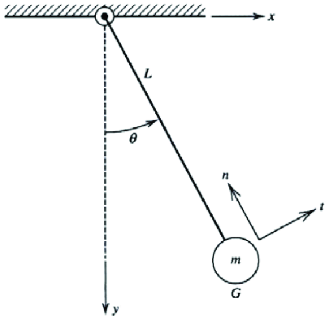
\includegraphics[width=0.8\linewidth]{pend}
		\caption{Náčrt kyvadla}
		\label{fig:pendulum}
	\end{figure}
	
\end{center}
 
\newpage
\section{Spustenie}
GUI bolo vytvorené v programe Matlab verzia 2018b. Spustenie je teda nutné vykonať priamo z Matlabu 2018b alebo \textbf{novšej} verzie. 
\subsection{Postup č. 1}
\begin{enumerate}
	\item Spustite program \textit{Matlab}.
	\item \textit{Current Folder} nastavte na priečinok, v ktorom sa nachádza súbor s názvom \textit{KyvGui.mlapp} (\cref{fig:spustenie}). 
	\begin{figure}[h!]
		\centering
		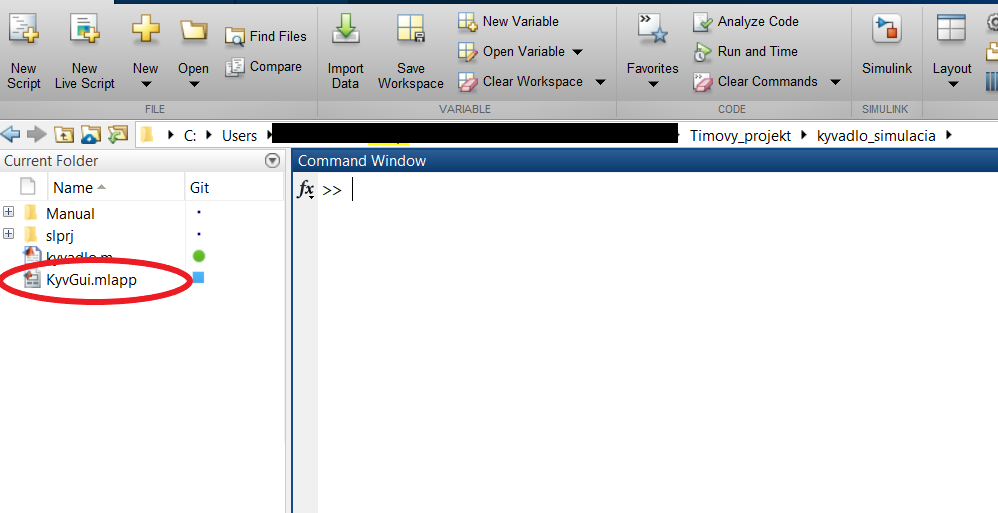
\includegraphics[width=0.9\linewidth]{spustenie1}
		\caption{Spustenie postup 1.}
		\label{fig:spustenie}
	\end{figure}
	\item Dvojklikom na \textit{KyvGui.mlapp} (zvýraznená položka na \cref{fig:spustenie}) spustíte GUI.
	
\end{enumerate}

\subsection{Postup č. 2 - editovanie}
\begin{enumerate}
	\item Spustite program \textit{Matlab}.
	\item \textit{Current Folder} nastavte na priečinok, v ktorom sa nachádza súbor s názvom \textit{KyvGui.mlapp} (\cref{fig:spustenie}).
	\item Do \textit{Command Window} napíšte príkaz \textit{>>appdesigner}. A stlačte Enter. Týmto príkazom ste spustili nástroj na tvorbu a \underline{editovanie} GUI (\cref{fig:spustenie2}).
	\begin{figure}[h!]
		\centering
		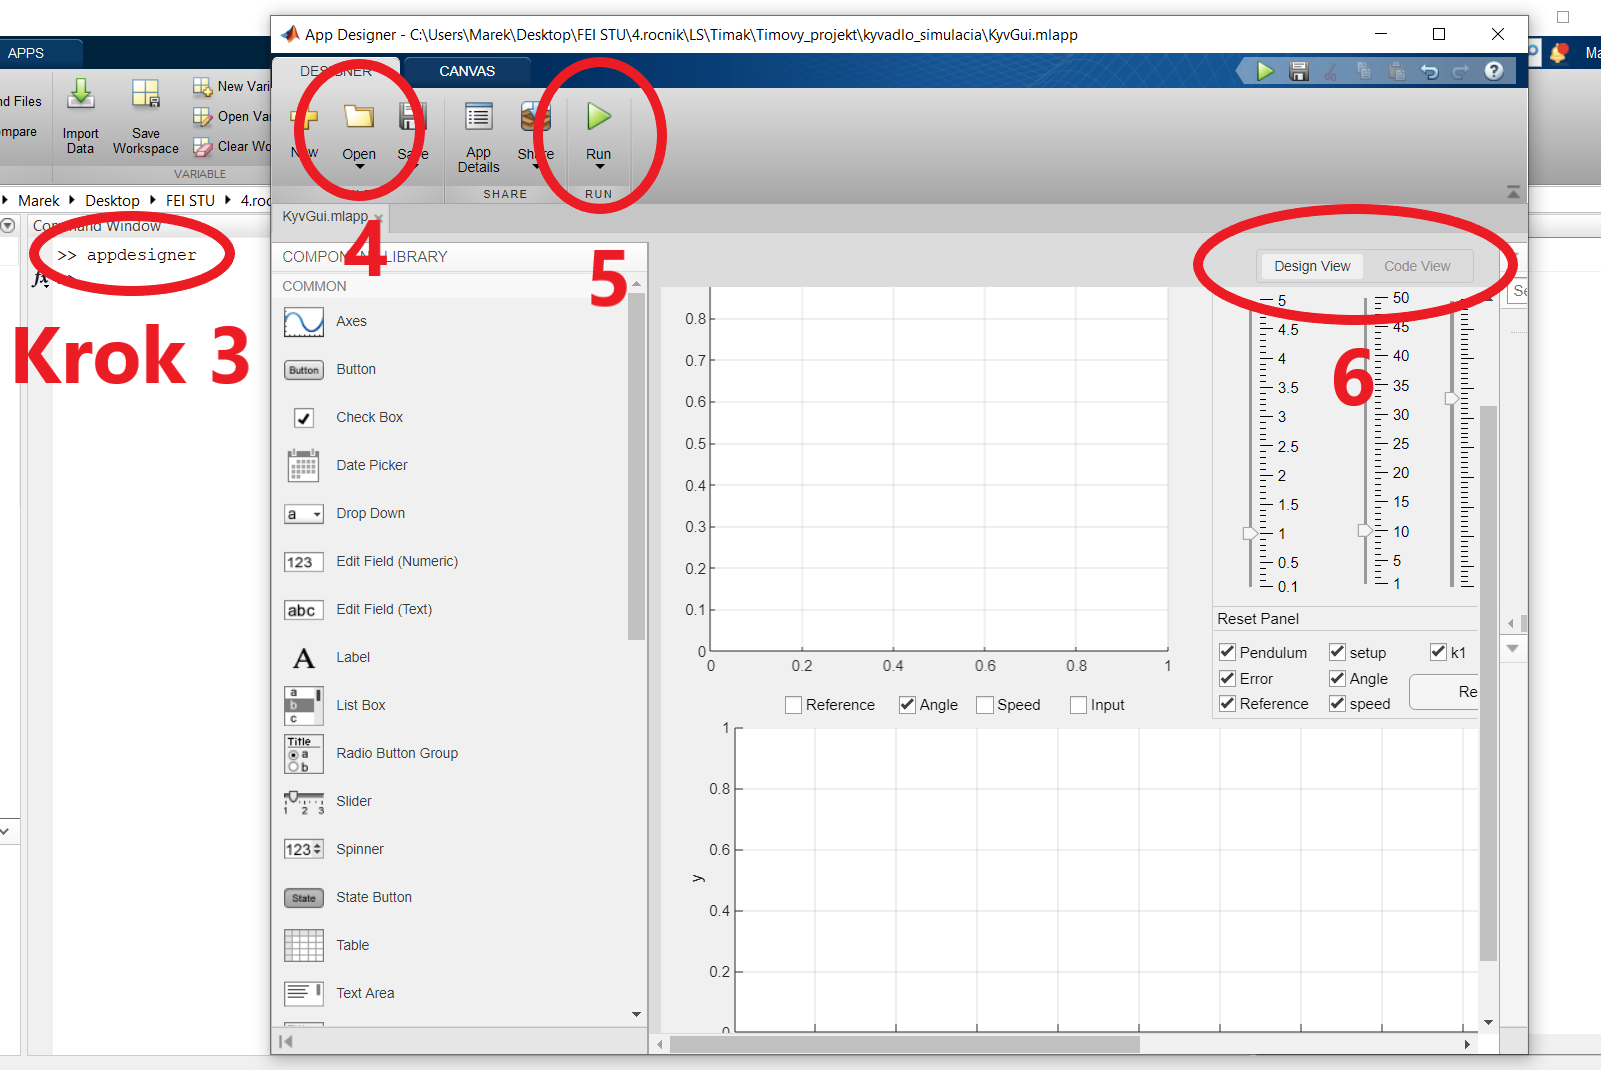
\includegraphics[width=0.9\linewidth]{spustenie2}
		\caption{Spustenie postup 2.}
		\label{fig:spustenie2}
	\end{figure}
    \item V hornej lište pomocou položky  \textit{Open} otvorte súbor \textit{KyvGui.mlapp}
    \item Potom pomocou položky  \textit{Run} spustíte GUI.
	\item Pomocou položky č. 6 môžete prepínať medzi zobrazením vzhľadu GUI a kódu GUI.
\end{enumerate}

\newpage
\section{Štruktúra GUI}
Po úspešnom spustení by ste mali vidieť nasledovné okno ako na \cref{fig:gui}.
	\begin{figure}[h!]
	\centering
	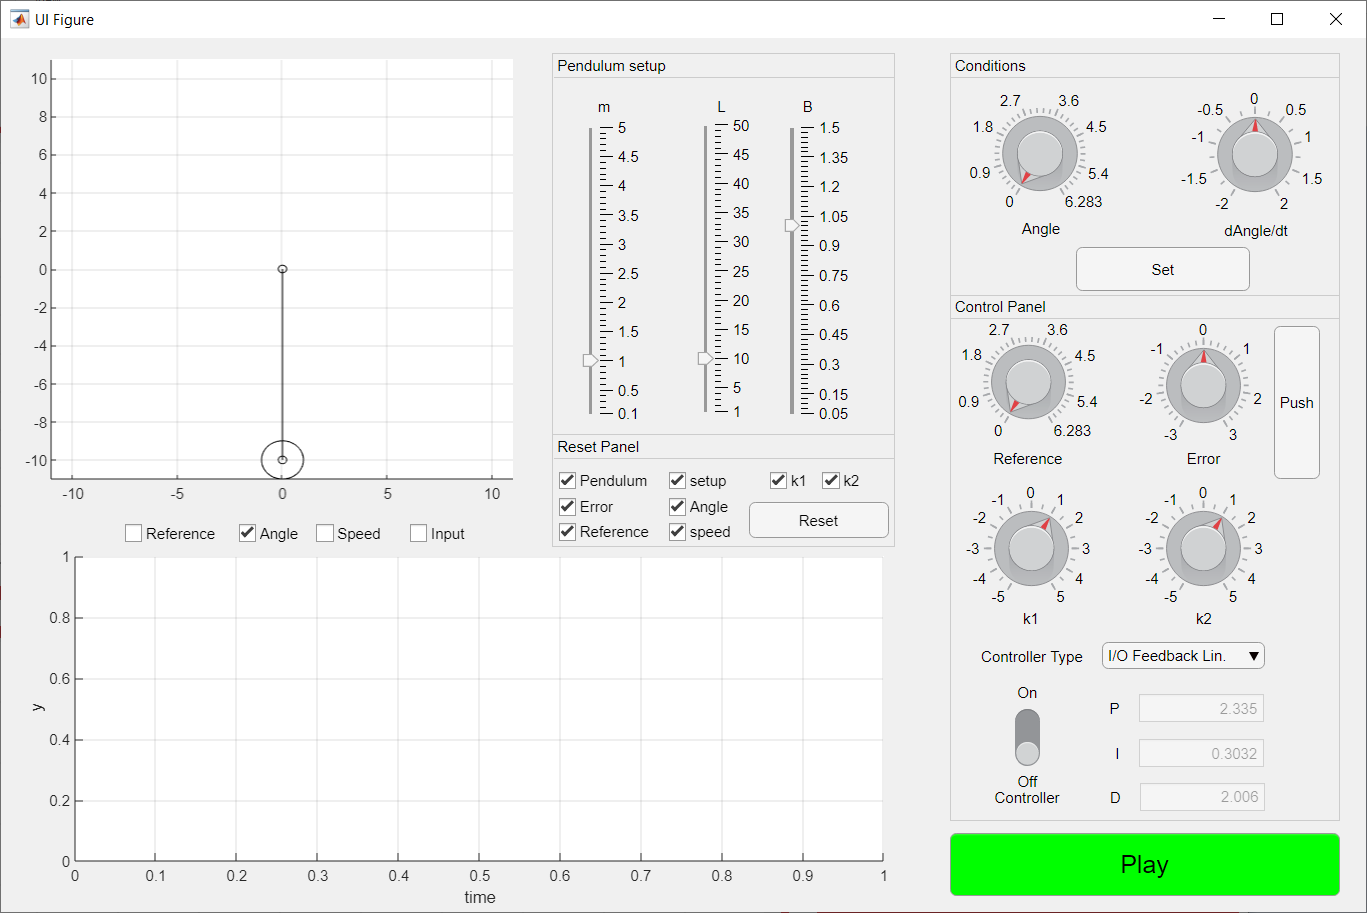
\includegraphics[width=0.9\linewidth]{gui}
	\caption{GUI}
	\label{fig:gui}
\end{figure}
Keďže GUI obsahuje relatívne veľa ovládacích prvkov, je rozčlenené na niekoľko panelov (skupín ovládacích prvkov, \cref{fig:structgui}). 

\subsection{Zoznam panelov}
\begin{enumerate}
	\item Okno animácie kyvadla.
	\item Okno priebehov veličín v čase.
	\item Panel výberu zobrazenia priebehov.
	\item Panel nastavenia fyzikálnych vlastností kyvadla.
	\item Panel resetovania nastavení.
	\item Panel nastavenia stavových veličín kyvadla.
	\item Panel riadenia.
	\item Tlačidlo \textbf{Play/Pause}.
\end{enumerate}

\makeatletter
\setlength{\@fptop}{0pt}
\makeatother

\begin{figure}[t!]
	\centering
	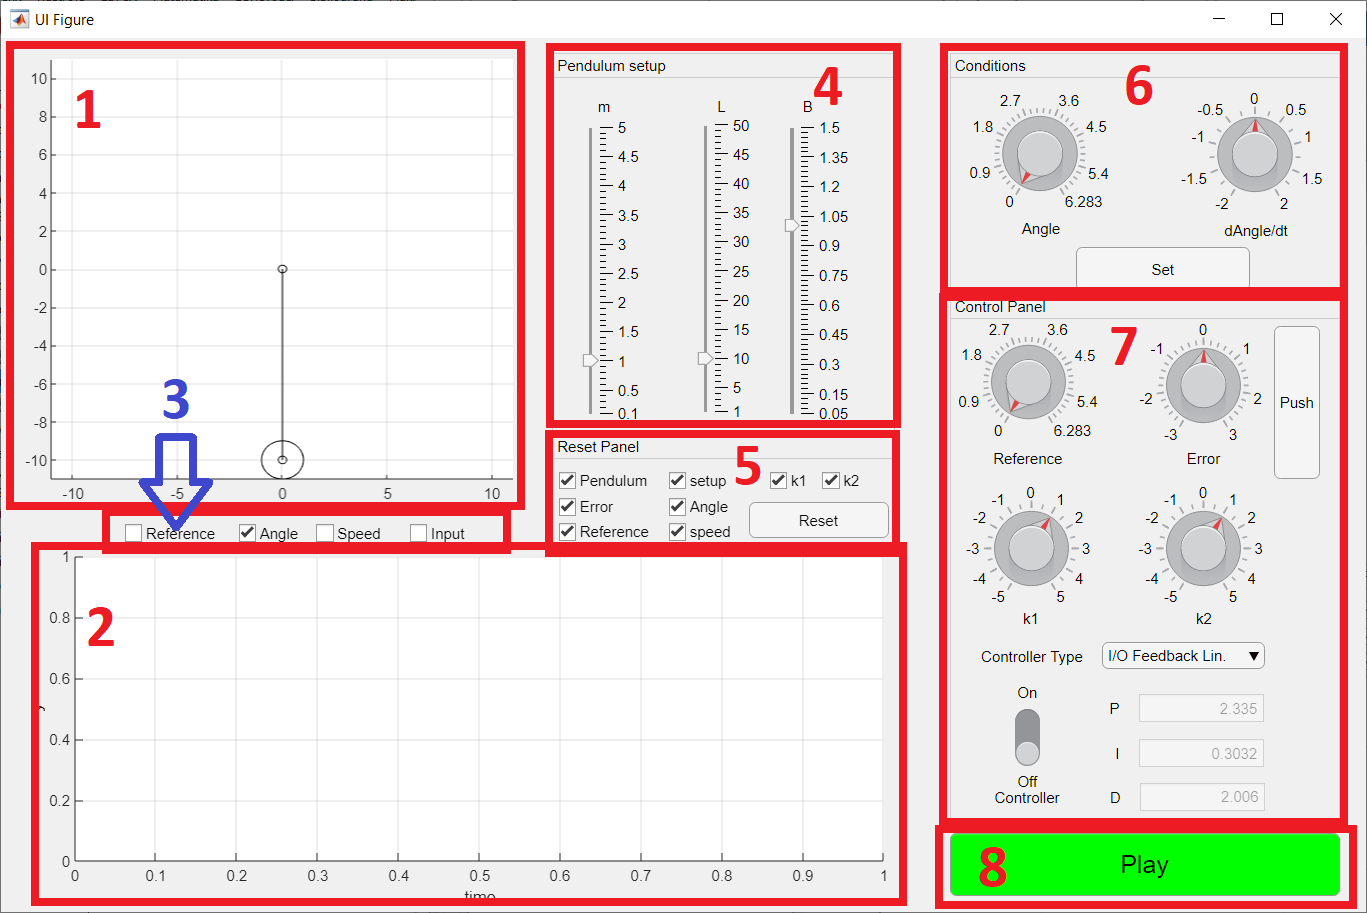
\includegraphics[width=0.9\linewidth]{structgui}
	\caption{Štrukturovanie GUI}
	\label{fig:structgui}
\end{figure}
 
 
\clearpage
\section{Ovládacie prvky}
 V tejto kapitole sa podrobnejšie pozrieme na funkcionalitu jednotlivých ovládačov, ktoré vidíme na \cref{fig:gui}  alebo \cref{fig:structgui} kde vidíme komponenty číslene označené, na toto označenie komponentov sa budeme odvolávať v celej kapitole. 
 \subsection{Animácia kyvadla} 
 Prvým komponentom  s označením \textbf{1} na \cref{fig:structgui} je graf, v ktorom sa pohybuje kyvado. Záves je upevnený v bode [0,0] a dĺžka závesu sa priamo viaže na parameter nastaviteľný v komponente č. \textbf{4}.
 	\begin{figure}[h!]
 	\centering
 	\includegraphics[width=0.9\linewidth]{kyv}
 	\caption{Komponent 1 - animácia kyvadla.}
 	\label{fig:kyv}
 \end{figure}
 \subsection{Priebehy a zobrazovanie veličín}
 V tejto podkapitole sme spojili kompnenty \textbf{2} a \textbf{3}. V komponente \textbf{2}, teda v grafe sa zobrazujú signály, vybraté v komponente \textbf{3}. 
 Používateľ si môže kombinovať zobrazenie výchylky (\textit{Angle}), uhlovej rýchlosti (\textit{Speed}) kyvadla, akčného zásahu (\textit{Input}) a želanej výchylky (\textit{Reference}) kyvadla ľubovolne podľa potreby. Na \cref{fig:prieb} je zobrazený uhol a želaná hodnota. Zobrazuje sa vždy posledných 800 časových úsekov. 
 	\begin{figure}[h!]
 	\centering
 	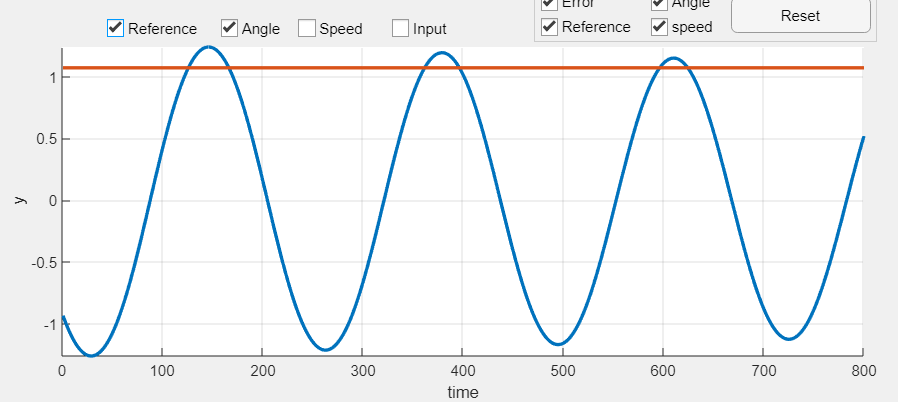
\includegraphics[width=0.9\linewidth]{priebehy}
 	\caption{Zobrazenie signálov.}
 	\label{fig:prieb}
 \end{figure}
\newpage
 \subsection{Vlastnosti kyvadla}
 Panel \textbf{4} umožňuje nastavenie fyzikálnych vlastností kyvadla. Konkrétne hmotnosť (\textit{m}), dĺžku závesu (\textit{L}) a tlmenie kmitov (\textit{B}). Nastavenie je realizované posuvníkmi v určitom rozmedzí hodnôt. Zmena nastavenia sa \underline{neprejavuje} súčasne s pohybom posuvníka, ale až po jeho uvoľnení sa pri najbližšom prekreslení aplikujú a zobrazia zmeny, čo môže chvíľku (cca. do 1 sekundy) trvať.
  	\begin{figure}[h!]
 	\centering
 	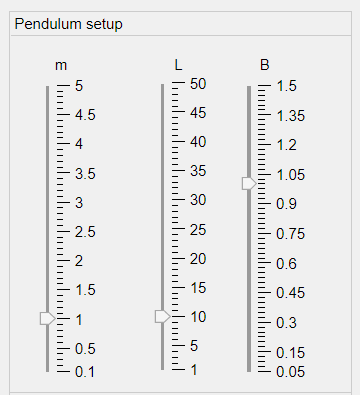
\includegraphics[width=0.7\linewidth]{fyz}
 	\caption{Nastavenie vlastností kyvadla.}
 	\label{fig:fyz}
 \end{figure}
 
  
 \subsection{Reset simulácie}
 Gui umožňuje reset nastavení na pôvodné hodnoty (pôvodné hodnoty - rozumej hodnoty pri spustení). Zaškrtnuté položky sa resetnú po stlačení tlačidla \textit{Reset} umiestnenom na tomto paneli.
 \begin{enumerate}
 	\item \textit{Pendulum} - nastaví aktuálnu rýchlosť a výchylku kyvadla na 0.
 	\item \textit{Error} - nastaví ovládač \textit{Error} v komponente \textbf{7} na 0.
 	\item \textit{Reference} - nastaví želanú hodnotu aj ovládač \textit{Reference} v paneli \textbf{7} na 0.
 	\item \textit{setup} - zresetuje hodnoty v komponente \textbf{4}.
 	\item \textit{Angle} - nastaví ovládač \textit{Angle} v komponente \textbf{6} na 0.
 	\item \textit{Speed} - nastaví ovládač \textit{Speed} v komponente \textbf{6} na 0.
  	\item \textit{k1, k2} - nastavia ovládače \textit{k1, k2} v komponente \textbf{7} na 1.
 \end{enumerate}
   	\begin{figure}[h!]
 	\centering
 	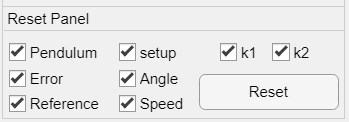
\includegraphics[width=0.7\linewidth]{reset}
 	\caption{Reset panel.}
 	\label{fig:reset}
 \end{figure}
 \subsection{Nastavenie stavov kyvadla}
 Panel \textbf{6} slúži na nastavenie výchylky a uhlovej rýchlosti kyvadla. Postup pri nastavení je nasledovný: Na otočných ovládačoch nastavte požadované hodnoty a stlačte tlačidlo \textit{Set}. Ak ste zmenili uhol to sa na animácii prejaví okamžite po slačení \textit{Set}. Pozorovať nastavenie rýchlosti je možné len pri bežiacej simulácii.
 
  \begin{figure}[h!]
 	\centering
 	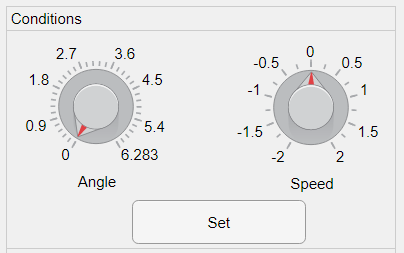
\includegraphics[width=0.7\linewidth]{cond}
 	\caption{Nastavenie stavov kyvadla.}
 	\label{fig:cond}
 \end{figure}
 
 \subsection{Riadiaci panel}
 Na \cref{fig:control} vidíme detail na komponent \textbf{7}. Skladá sa z nasedovných ovládačov:
 \begin{enumerate}
 	\item \textit{Reference} - nastavuje želanú hodnotu výchylky kyvadla. Nastavenie sa uskutočnuje súčasne s pohybom ovládača, teda netreba žiadnym tlačidlom potrvdzovať nastavenie hodnoty. 
 	\item \textit{Error} - porucha, simuluje udelenie rýchlosti kyvadlu vonkajšou silou tzv. šťuchnutie/úder. Ovládačom \textit{Error} sa nastavuje veľkosť/sila úderu a až stlačením tlačidla \textit{Push} sa vykoná. 
 	\item \textit{k1, k2} - nastavujú parametre \textit{k1, k2}, ktoré sa využívajú pri riadení pomocou spätnoväzbovej linearizácií. Pri použití iných regulátorov sú  tieto ovládače deaktivované.
 	\item \textit{Controller Type} - dropdown menu, ktoré umožnuje výber (\cref{fig:list}) regulátora použitého pre riadenie kyvadla. Pri spustení je vždy zvolený regulátor odvodený vstupno-výstupnou spätnoväzbovou linearizáciou. Pre položku \textit{PID} je použitý klasický PID regulátor s prednastavenými hodnotami. Tieto hodnoty sú zobrazené v textových oknách \textit{P, I, D} napriek tomu, že sú neaktívne. 	
 \begin{figure}[h!]
	\centering
	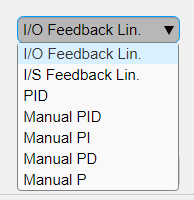
\includegraphics[width=0.6\linewidth]{list}
	\caption{Menu s regulátormi.}
 	\label{fig:list}
 \end{figure}

 	\item \textit{P, I, D} - textové okná určené pre vloženie hodnoty používteľom. Aktivujú sa len pri zapnutí niektorého z manuálnych reguátorov (\cref{fig:manualPID}). Inak sú neaktívne ako na \cref{fig:control}.
 	 \begin{figure}[h!]
 		\centering
 		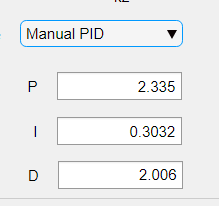
\includegraphics[width=0.6\linewidth]{manualPID}
 		\caption{Menu s regulátormi.}
 		\label{fig:manualPID}
 	\end{figure}
 
    \item \textit{Controller} - prepínač \textbf{nadradený} všetkým predchádzajúcim nastaveniam, slúži na odpojenie regulátora. Inak povedané akčný zásah bude \textbf{nulový}. Treba dbať na to, aby bol v polohe \textbf{\textit{ON}}, keď je to žiadúce.
 

 \end{enumerate} 

\makeatletter
\setlength{\@fptop}{0pt}
\makeatother
   \begin{figure}[h!]
 	\centering
 	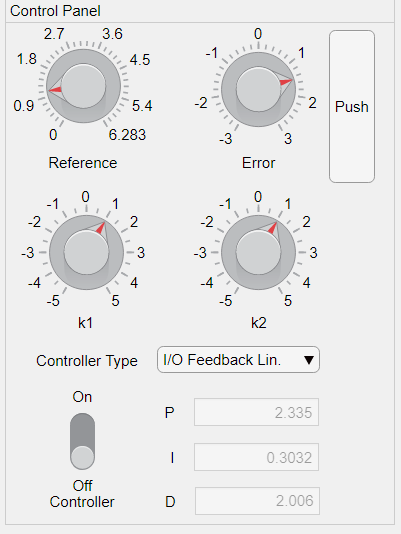
\includegraphics[width=0.9\linewidth]{control}
 	\caption{Control panel.}
 	\label{fig:control}
 \end{figure}
\clearpage
 \subsection{Spustenie/Pozastavenie simulácie}  
  Komponentom \textbf{8} je najväčšie tlačidlo v pravom dolnom rohu. Slúži na ovládanie behu simulácie. Má 2 stavy.
  \begin{enumerate}
  	\item Je zelené a je na ňom napísanie play (\cref{fig:play}), vtedy je simulácia pozastavená a stlačením tlačidla ju spustíte.
  	\item Je žlté a je na ňom napísanie pause (\cref{fig:pause}), vtedy je simulácia pustená a stlačením tlačidla ju pozastavíte.
  \end{enumerate} 
   	 \begin{figure}[h!]
  	\centering
  	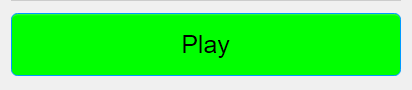
\includegraphics[width=0.6\linewidth]{play}
  	\caption{Play pre spustenie.}
  	\label{fig:play}
  \end{figure}  

   	 \begin{figure}[h!]
	\centering
	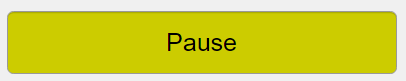
\includegraphics[width=0.6\linewidth]{pause}
	\caption{Pause pre pozastavenie.}
	\label{fig:pause}
\end{figure} 

\section{Ukončenie programu}
Pri zatváraní programu, naprv pozastavte simulovanie (tlačidlo v stave ako na \cref{fig:play}) a až potom zatvore symbolom \textit{X} v pravom hornom rohu. Ak tak vykonáte počas behu simulácie Matlab bude hlásiť chyby, ktoré môžu znepokojiť užívateľa.

\end{document}